% Copyright 2004 by Till Tantau <tantau@users.sourceforge.net>.
%
% In principle, this file can be redistributed and/or modified under
% the terms of the GNU Public License, version 2.
%
% However, this file is supposed to be a template to be modified
% for your own needs. For this reason, if you use this file as a
% template and not specifically distribute it as part of a another
% package/program, I grant the extra permission to freely copy and
% modify this file as you see fit and even to delete this copyright
% notice. 



\documentclass[xcolor={table,dvipsnames,usenames}]{beamer}
\usepackage{empheq}
\usepackage{color}
\definecolor{myblue}{rgb}{.8, .8, 1}
\newlength\mytemplen
\newsavebox\mytempbox

\makeatletter
\newcommand\mybluebox{%
	\@ifnextchar[%]
	{\@mybluebox}%
	{\@mybluebox[0pt]}}

\def\@mybluebox[#1]{%
	\@ifnextchar[%]
	{\@@mybluebox[#1]}%
	{\@@mybluebox[#1][0pt]}}

\def\@@mybluebox[#1][#2]#3{
	\sbox\mytempbox{#3}%
	\mytemplen\ht\mytempbox
	\advance\mytemplen #1\relax
	\ht\mytempbox\mytemplen
	\mytemplen\dp\mytempbox
	\advance\mytemplen #2\relax
	\dp\mytempbox\mytemplen
	\colorbox{myblue}{\hspace{1em}\usebox{\mytempbox}\hspace{1em}}}

\makeatother
%\usepackage[utf8]{hyperref}
%\hypersetup{
%	colorlinks=true,
%	linkcolor=blue,
%	filecolor=magenta,      
%	urlcolor=cyan,
%}
% There are many different themes available for Beamer. A comprehensive
% list with examples is given here:
% http://deic.uab.es/~iblanes/beamer_gallery/index_by_theme.html
% You can uncomment the themes below if you would like to use a different
% one:
%\usetheme{AnnArbor}
%\usetheme{Antibes}
%\usetheme{Bergen}
%\usetheme{Berkeley}
%\usetheme{Berlin}
%\usetheme{Boadilla}
%\usetheme{boxes}
%\usetheme{CambridgeUS}
%\usetheme{Copenhagen}
%\usetheme{Darmstadt}
%\usetheme{default}
%\usetheme{Frankfurt}
%\usetheme{Goettingen}
%\usetheme{Hannover}
%\usetheme{Ilmenau}
%\usetheme{JuanLesPins}
%\usetheme{Luebeck}
\usetheme{Madrid}
%\usetheme{Malmoe}
%\usetheme{Marburg}
%\usetheme{Montpellier}
%\usetheme{PaloAlto}
%\usetheme{Pittsburgh}
%\usetheme{Rochester}
%\usetheme{Singapore}
%\usetheme{Szeged}
%\usetheme{Warsaw}
%gets rid of bottom navigation bars
%\setbeamertemplate{footline}[frame number]{}

%gets rid of bottom navigation symbols
\setbeamertemplate{navigation symbols}{}
%\usepackage[dvipsnames]{xcolor}
%gets rid of footer
%will override 'frame number' instruction above
%comment out to revert to previous/default definitions
%\setbeamertemplate{footline}{}
\setbeamertemplate{footline}[page number]


\title{Hardness vs. Randomness}

% A subtitle is optional and this may be deleted
%\subtitle{Optional Subtitle}

\author{Rahul Gupta\inst{1}, 
	Shubham Sharma\inst{1}}
% - Give the names in the same order as the appear in the paper.
% - Use the \inst{?} command only if the authors have different
%   affiliation.

\institute[Universities of Somewhere and Elsewhere] % (optional, but mostly needed)
{
  \inst{1}%
  Indian Institute of Technology Kanpur, India}
% - Use the \inst command only if there are several affiliations.
% - Keep it simple, no one is interested in your street address.

\date{18 April 2019}
% - Either use conference name or its abbreviation.
% - Not really informative to the audience, more for people (including
%   yourself) who are reading the slides online

%\subject{Theoretical Computer Science}
% This is only inserted into the PDF information catalog. Can be left
% out. 

% If you have a file called "university-logo-filename.xxx", where xxx
% is a graphic format that can be processed by latex or pdflatex,
% resp., then you can add a logo as follows:

% \pgfdeclareimage[height=0.5cm]{university-logo}{university-logo-filename}
% \logo{\pgfuseimage{university-logo}}

% Delete this, if you do not want the table of contents to pop up at
% the beginning of each subsection:
%\AtBeginSubsection[]
%{
%  \begin{frame}<beamer>{Outline}
%    \tableofcontents[currentsection,currentsubsection]
%  \end{frame}
%}
\usepackage[font=scriptsize,skip=4pt]{caption}
\usepackage{multirow}
\usepackage{color, colortbl}
\definecolor{LightCyan}{rgb}{0.88,1,1}
\definecolor{darkblue}{rgb}{0.0,0.0,1}
\hypersetup{colorlinks,breaklinks,linkcolor=darkblue,urlcolor=darkblue,anchorcolor=darkblue,citecolor=darkblue}
% Let's get started
\begin{document}

\newcommand{\ddnnf}{\ensuremath{\mathsf{dag}}}
\newcommand{\WAPS}{\ensuremath{\mathsf{WAPS}}}
\newcommand{\KUS}{\ensuremath{\mathsf{KUS}}}
\newcommand{\DSPACE}{\ensuremath{\mathsf{DSPACE}}}
\newcommand{\RNC}{\ensuremath{\mathsf{RNC}}}
\newcommand{\BPP}{\ensuremath{\mathsf{BPP}}}
\newcommand{\DTIME}{\ensuremath{\mathsf{DTIME}}}
\newcommand{\RTIME}{\ensuremath{\mathsf{RTIME}}}
\newcommand{\WeightGen}{\ensuremath{\mathsf{WeightGen}}}
\newcommand{\prob}{\ensuremath{\mathsf{Pr}}}
\newcommand{\UniGen}{\ensuremath{\mathsf{UniGen2}}}
\newcommand{\satisfying}[1]{\ensuremath{R_{#1}}} %
\newcommand{\satisfyingv}[2]{\ensuremath{R_{#1\downarrow #2}}}
\newcommand{\Sampler}{\ensuremath{\mathsf{Sampler}}}
\newcommand{\sampleList}{\ensuremath{\mathsf{SampleList}}}
\newcommand{\Shuffle}{\ensuremath{\mathsf{Shuffle}}}
\newcommand{\Append}{\ensuremath{\mathsf{Append}}}
\newcommand{\Stitch}{\ensuremath{\mathsf{Stitch}}}
\newcommand{\IS}{\ensuremath{\mathsf{IS}}}
\newcommand{\normalize}{\ensuremath{\mathsf{Normalize}}}
\newcommand{\WCounter}{\ensuremath{\mathsf{WAnnotate}}}
\newcommand{\PCompile}{\ensuremath{\mathsf{PCompile}}}

\definecolor{ao(english)}{rgb}{0.0, 0.5, 0.0}

\begin{frame}
  \titlepage
  \begin{center}
  	\footnote{\href{https://www.math.ias.edu/avi/node/780}{https://www.math.ias.edu/avi/node/780}}
%  	The tool is available online \href{https://github.com/meelgroup/WAPS}{\textcolor{blue}{https://github.com/meelgroup/WAPS}}
  \end{center}
  
\end{frame}

\section{Pseudorandom Generator}
\begin{frame}{Pseudorandom Generator (PRG)}
\begin{itemize}
	\item $G: \{0,1\}^r \rightarrow \{0,1\}^n$ is a {\underline{pseudorandom generator}} such that it \textcolor{red}{appears random (fools)} to a \textcolor{blue}{class of test functions}.
	\pause
	\item $G~\epsilon$-fools $F$ if $\forall f \in F$ such that $f: \{0,1\}^n \rightarrow \{0,1\}$
	$$\Big|\prob\big[f(y)\big] -  \prob\big[f(G(x))\big]\Big| \leq \epsilon$$
	where $x$ is choosen uniformly from $\{0,1\}^r$ and $y$ from $\{0,1\}^n$
	\pause
	\begin{itemize}
		\item[--] Parity-function.
		\item[--] Polynomial-funtions.
		\item[--] \textcolor{blue}{Boolean-circuits}.
	\end{itemize}
	\pause
	\item G is a \textcolor{blue}{quick pseudorandom generator} if it runs in \underline{deterministic} time \textcolor{red}{exponential} in its input size, $G \in \DTIME (2^{O(r)})$.
	\begin{itemize}
		\item[--] \textcolor{blue}{quality of the output} -- $n,\epsilon$
		\item[--] \textcolor{blue}{price} -- $r$
	\end{itemize}
\end{itemize}
\end{frame}
\begin{frame}{Motivation}
\begin{itemize}
	\item If there exists a quick pseudorandom generator $G: \log(n) \rightarrow n$ then for any time constructible bound $t=t(n):$ $$\RTIME(t) \subset \DTIME(2^{O(\log(t^2))})$$
	\pause
	\begin{center}
			        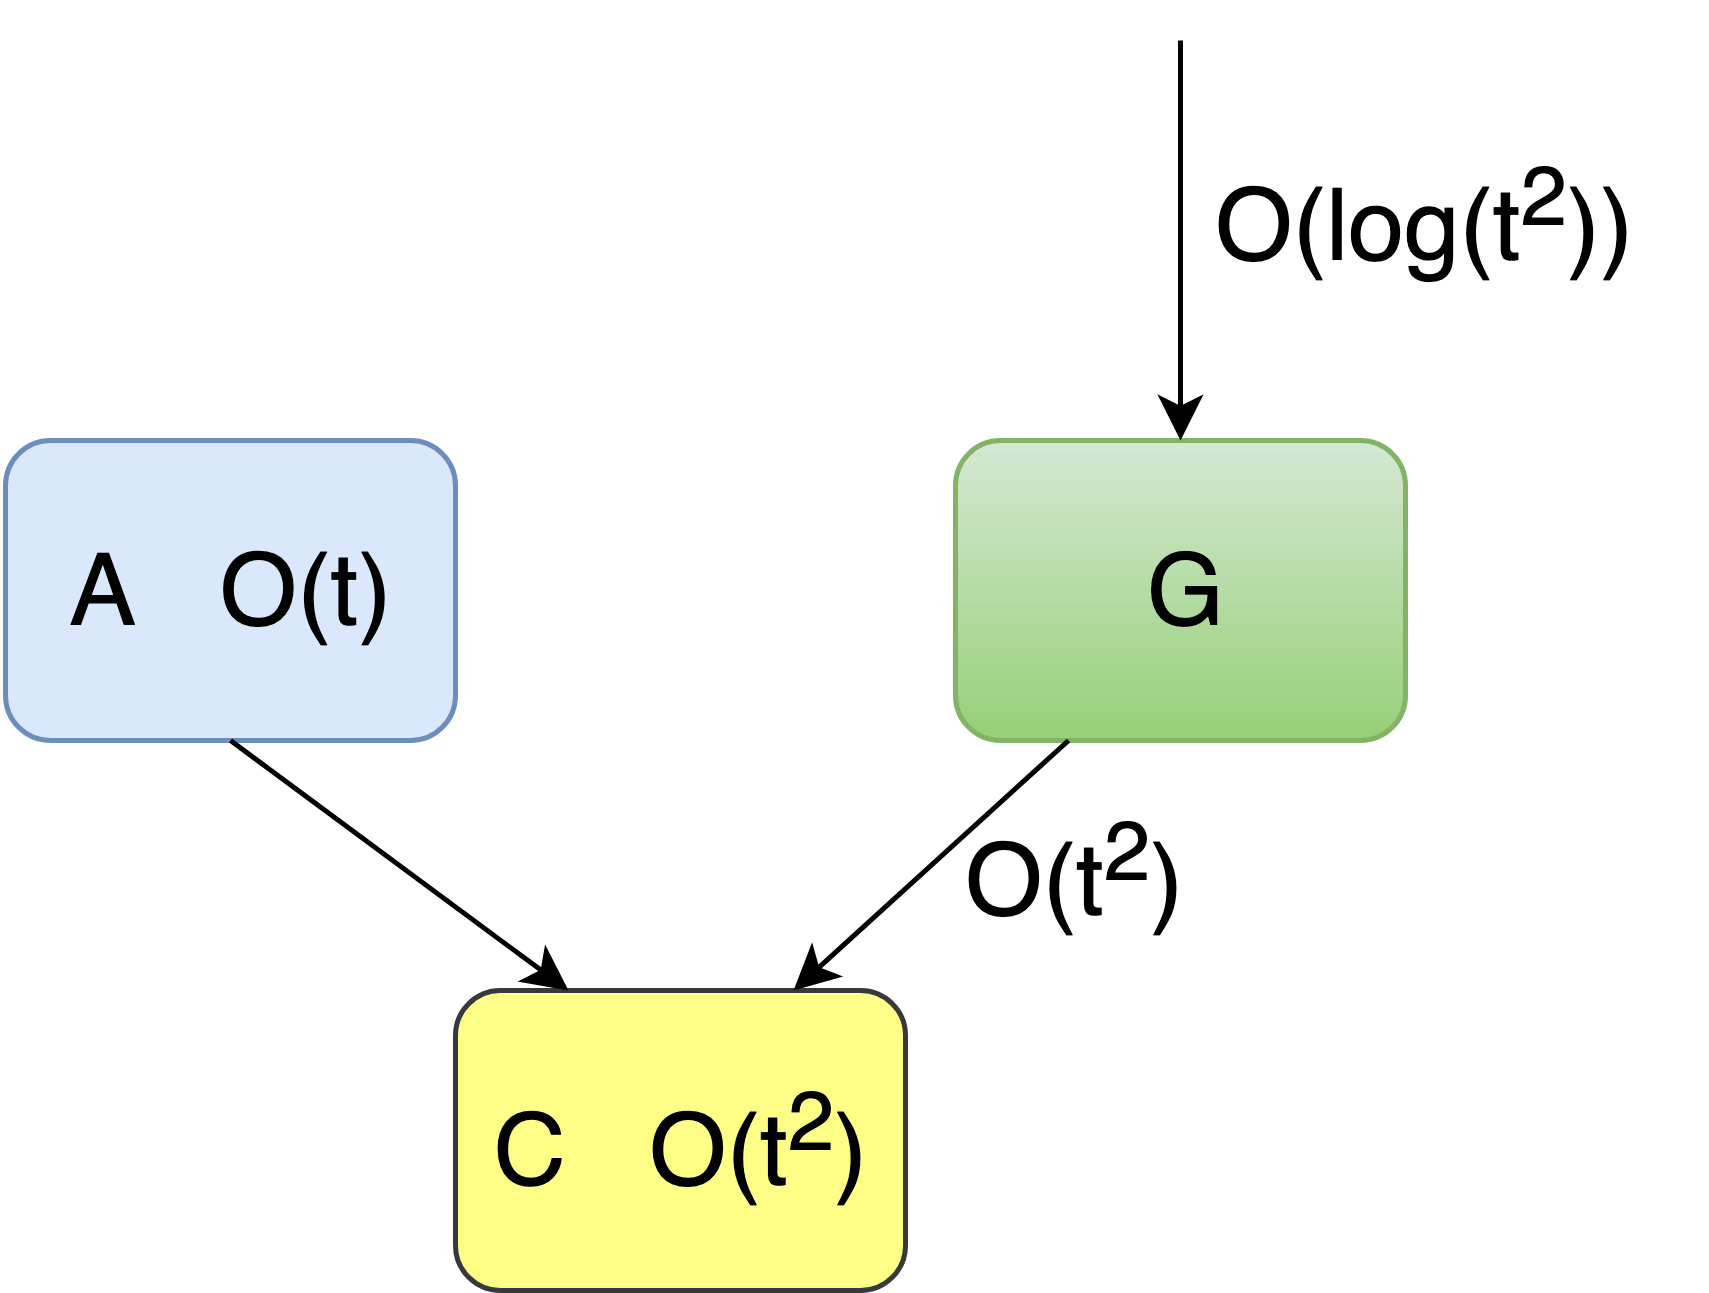
\includegraphics[width=0.4\columnwidth]{figures/RandomSimulation}
	\end{center}
\pause
\item  Simulate $A$ deterministically, by trying all the possible random seeds and taking a majority vote. 
\end{itemize}
\end{frame}
\begin{frame}{Applications}
	\begin{minipage}[b]{0.3\textwidth}
	        \begin{center}
		        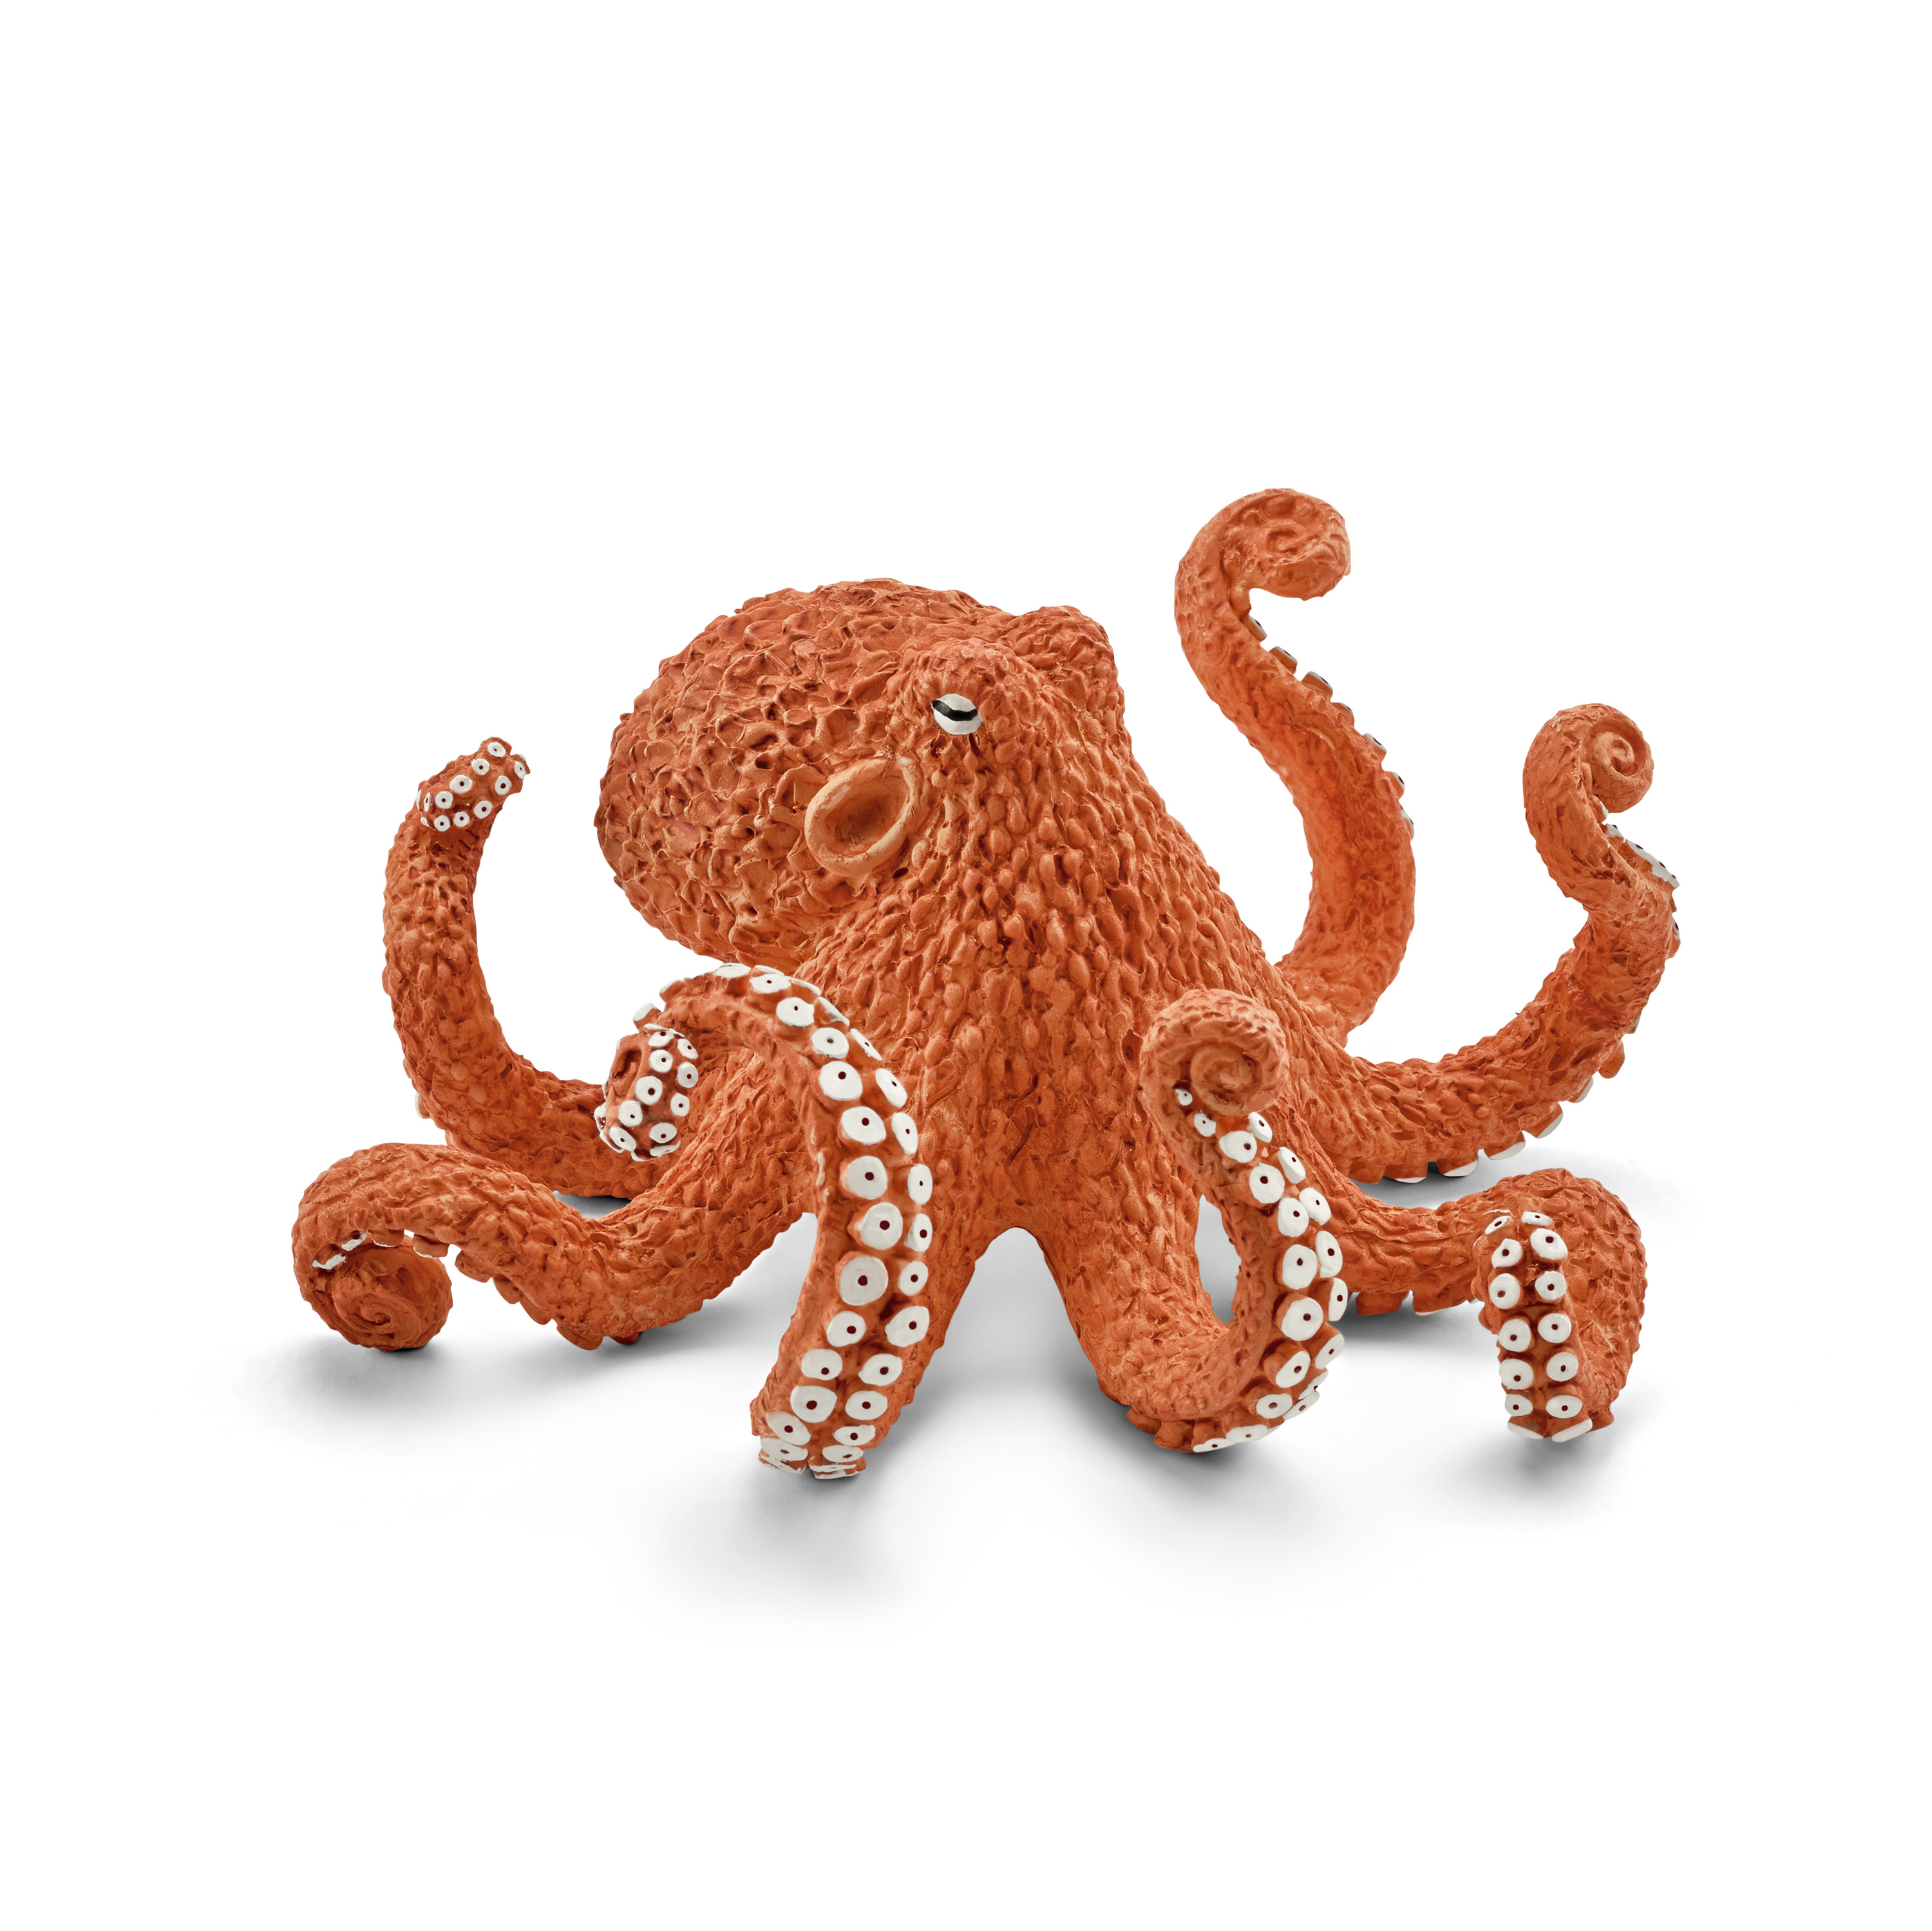
\includegraphics[width=\columnwidth]{figures/octopus.jpg}
	        \end{center}
	 \end{minipage}
 \begin{minipage}[b]{0.65\textwidth}
 	        \begin{itemize}
				\item $\BPP \subset	\cap_{\epsilon > 0}	\DTIME (2^{n^{\epsilon}})$
				\pause
				\item   $\BPP \subset \DTIME (2^{(\log n)^{c}})$
				\pause
				\item $\BPP = P$
				\pause
				\item $\RNC \subset\cap_{\epsilon > 0}	\DSPACE ({n^{\epsilon}})$
				\pause 
				\item $\RNC \subset \DSPACE(polylog)$\\
				\quad \quad \vdots
 	        \end{itemize}
 	    \end{minipage} 
\end{frame}
%	\begin{minipage}[b]{0.3\textwidth}
%        \begin{center}
%%	        \includegraphics[width=\columnwidth]{figures/HardwareValidation}
%        \end{center}
%    \end{minipage} 
%	\begin{minipage}[b]{0.65\textwidth}
%        \begin{itemize}
%            \item Design is simulated with test vector \\ (values of a and b)
%            \item Results from simulation compared to intended results
%            \item Challenge: How do we generate test vectors?
%                \begin{itemize}
%                    \item[--] $2^{128}$ combinations for a toy circuit
%                \end{itemize}
%            \item Use constraints to represent interesting verification scenarios
%            %\item Use weight distribution to meet the coverage goals
%        \end{itemize}
%    \end{minipage}
%\end{frame}
%\begin{frame}{Constrained Simulation}
%
%	\begin{minipage}[b]{0.3\textwidth}
%        \begin{center}
%%	        \includegraphics[width=\columnwidth]{figures/HardwareValidation}
%        \end{center}
%    \end{minipage} 
%	\begin{minipage}[b]{0.65\textwidth}
%        \begin{itemize}
%            \item {\bf Constraints}:
%                \begin{itemize}
%                    \item Designers:
%                        \begin{itemize}
%                            \item[--] $a +_{64} 11 *_{32} b = 12$
%                            \item[--] $a <_{64} (b >> 4)$
%                        \end{itemize}
%%                    \item Past Experience: 
%%                        \begin{itemize}
%%                            \item[--] $40 <_{64} 34 +_{64} a <_{64} 5050$
%%                            \item[--] $120 <_{64} b <_{64} 230$
%%                        \end{itemize}
%                    \item Users: 
%                        \begin{itemize}
%                            \item[--] $232 *_{32} a +_{64} b! = 1100$
%                            \item[--] $1020 <_{64} (b/_{64} 2) +_{64} a <_{64} 2200$
%                        \end{itemize}
%                \end{itemize}
%            \pause
%            \item {\bf Weight distribution}: Define $W(\cdot)$ over a subset of literals to perform directed testing
%            \item {\bf Test vectors}: sampled solutions of constraints conditioned on $W(\cdot)$
%        \end{itemize}
%    \end{minipage}
%\end{frame}
%
%
%\section{Sampling}
%
%%\subsection{First Subsection}
%
%\begin{frame}{Weighted and Projected Sampling}
%  \begin{itemize}
%  \item Given:
%  \begin{itemize}
%  	\item CNF formula $F$ over a set of variables $X$
%    \item Set of projecting variables $P \subseteq X$
%    \item Weight function $W(\cdot)$ over literals
%        \begin{itemize}
%            \item[--] The weight of assignment is the product of weights of its literals
%        \end{itemize}
%  \end{itemize}
%	\pause
%  \item Weighted and Projected Sampler:
%  \begin{empheq}[box={\mybluebox[5pt]}]{equation*}
%	\forall y \in \satisfyingv{F}{P}, \prob\left[y \text{ is output }\right] = \frac{W(y)}{W(\satisfyingv{F}{P})}
%  \end{empheq}
%%  \framebox[]{\forall y \in \satisfyingv{F}{P}, \prob\left[y \text{ is output }\right] = \frac{W(y)}{W(\satisfyingv{F}{P})}}
%  \end{itemize}
%\end{frame}
%
%\begin{frame}{Applications of Weighted and Projected Sampling}
%%\begin{itemize}
%	\begin{figure}
%		\centering
%%		\includegraphics[width=0.75\columnwidth]{figures/image223.png}
%		%   \captionof{figure}{A figure}
%		\label{fig:test1}
%	\end{figure}
%%	\item Hardware Validation
%%	\item Probabilistic Reasoning 
%%	\item Machine Learning
%%	\item Statistical Physics
%%	\item Used for generating stimuli for Hardware Verification. Designers often test their hardware by constraining input using expert knowledge rules and modeling hardware into a constraint satisfaction problem where assignments satisfy a weight distribution.
%%	\item Used in Probabilistic Reasoning to generate samples from a Bayesian Network conditioned upon an evidence.
%%	\begin{itemize}
%%		\item[--] Bayesian Network can be encoded to a literal-weighted CNF.
%%		\item[--] The weights of literals representing the evidence can be appropriately set.
%%	\end{itemize}
%%	 where probabilities are encoded in weights of literals. 
%%	Furthermore, likelihood weighted sampling (conditioned upon an evidence) can be done by setting appropriate weights
%%\end{itemize}
%\end{frame}
%\begin{frame}{Wish List}
%\begin{itemize}
%	\item Theoretical guarantee that samples projected over a sampling set satisfy a certain weight distribution
%	\item Scalability
%	\item Anytime Generation:
%	\begin{itemize}
%		\item[--] Testing typically involves multiple iterations of sampling and verification
%	\end{itemize}
%\end{itemize}
%\end{frame}
%\section{Prior Work}
%
%\begin{frame}{Prior Work}
%\textbf{Strong guarantees but poor scalability}
%\begin{itemize}
%    \item Hashing based techniques - {\WeightGen} \quad \hfill (\textcolor{blue}{Chakraborty et al. 2014} )
%	\item BDD based techniques \quad \hfill (\textcolor{blue}{Yuan et al. 1999, Yuan et al. 2004, Kukula \\ \quad \quad \quad \quad \quad \quad \quad \quad \quad \quad \quad \quad  and
%	Shiple 2000})
%\end{itemize}
%\pause
%\textbf{Weak guarantees but impressive scalability}
%\begin{itemize}
%	\item MCMC, Metropolis-Hasting (\textcolor{blue}{Jerrum et al. 1996, Mardras et al. '02})
%\end{itemize}
%\pause
%    \begin{center}
%    \textcolor{blue}{How to bridge this gap between theory and practice?}
%    \end{center}
%\end{frame}
%
%\begin{frame}{Close Cousins: Counting and Sampling}
%\begin{itemize}
%	\item Approximate counting and almost-uniform sampling are
%	inter-reducible \quad \quad \quad \quad \quad \quad \quad \quad \quad \quad	(\textcolor{blue}{Jerrum et al. 1986})
%	\item Can we design exact samplers that requires polynomial calls to an exact
%	counter?
%	\item Exact counting techniques based on DPLL exploration generate d-DNNF (\textcolor{blue}{Huang and Darwiche 2007})
%	\item Uniform sampling can be performed by making constant number of passes over compiled d-DNNF (\textcolor{blue}{Sharma et al. 2018})
%	\item Can knowledge compilation technique be used to perform weighted and projected sampling?
%\end{itemize}
%\end{frame}
%
%
%\begin{frame}{d-DNNF}
%The \underline{Deterministic Decomposable Negation Normal Form} (\textbf{d-DNNF})  is a strict subset of \textbf{NNF} that further imposes that the representation is:
%
%\begin{itemize}
%	\item {\bf Deterministic}: the operands of $\lor$ in all well-formed Boolean formula in the NNF are mutually inconsistent
%	
%	\item {\bf Decomposable}: the operands of $\land$ in all well-formed Boolean formula in the NNF are expressed in a mutually disjoint set of variables
%\end{itemize}
%
%\begin{figure}
%		\centering
%%		\includegraphics[width=.5\linewidth]{figures/dDNNF}
%		%   \captionof{figure}{A figure}
%		\label{fig:test1}
%\end{figure}
%\end{frame}
%
%\begin{frame}{An example of d-DNNF}
%\begin{figure}
%	\centering
%%	\includegraphics[width=.7\linewidth]{figures/4_4.eps}
%	%   \captionof{figure}{A figure}
%	\label{fig:test1}
%\end{figure}
%\end{frame}
%\begin{frame}{The power of d-DNNF}
%\begin{itemize}
%	\item Solutions can be enumerated in linear time in the size of d-DNNF
%	\begin{itemize}
%		\item [--] {\bf \textcolor{blue}{OR Node}}: Take union of the solutions of children
%		\item [--] {\bf \textcolor{blue}{AND Node}}: Take cross-product of the solutions of the children
%	\end{itemize}
%	\item Counting is linear time in the size of d-DNNF
%	\begin{itemize}
%		\item [--] {\bf \textcolor{blue}{OR Node}}:  Sum the solutions of children
%		\item [--] {\bf \textcolor{blue}{AND Node}}: Multiply the solutions of children
%	\end{itemize}
%\end{itemize}
%\end{frame}
%%\begin{frame}{An example of d-DNNF}
%%\begin{figure}
%%	\centering
%%	\includegraphics[width=.5\linewidth]{figures/d4.eps}
%%	%   \captionof{figure}{A figure}
%%	\label{fig:test1}
%%\end{figure}
%%\end{frame}
%\section{WAPS}
%\begin{frame}{WAPS}
%\begin{center}
%%	\includegraphics[width=\linewidth]{figures/waps.png}
%\end{center}
%\end{frame}
%
%\begin{frame}{WAPS}
%\begin{center}
%%	\includegraphics[width=\linewidth]{figures/waps1.pdf}
%\end{center}
%\end{frame}
%
%\begin{frame}{Projected Compilation}
%$F =  (x_6 \lor x_5 \lor \neg x_1 \lor x_3) \land (x_3 \lor  x_6 \lor \neg x_5 \lor \neg x_1) \land (\neg x_2 \lor x_4 \lor \neg x_1) \land  \text{}\quad\quad(x_1 \lor x_2)\land (x_3 \lor \neg x_6 \lor \neg x_1) \land (\neg x_3 \lor \neg x_5 \lor x_6)$
%
%${P = \{x_1,x_2,x_3\}}$
%\begin{center}
%%	\includegraphics[width=0.8\linewidth]{figures/compilation.png}
%\end{center}
%\end{frame}
%
%\begin{frame}{WAPS}
%\begin{center}
%%	\includegraphics[width=\linewidth]{figures/waps2.pdf}
%\end{center}
%\end{frame}
%
%\begin{frame}{Weight Annotation}
%\begin{center}	
%%	\includegraphics[height=3.5cm]{figures/WAnnotate.pdf}
%	\hfill
%%	\includegraphics[height=3.5cm]{figures/WAnnotate2.pdf}
%\end{center}	%		\captionof{figure}{Annotation at an AND Node}
%\end{frame}
%
%\begin{frame}{WAPS}
%\begin{center}
%%	\includegraphics[width=\linewidth]{figures/waps3.pdf}
%\end{center}
%\end{frame}
%
%\begin{frame}{Getting one sample}
%\begin{itemize}
%	\item Since, solutions are disjoint at different children of an OR node, to draw a sample, we can simply perform a Bernoulli experiment with probabilities proportional to the weights of children at OR node
%	\item At AND node, we simply stitch the samples from its children
%\end{itemize}
%\begin{center}
%%	\includegraphics[width=0.29\linewidth]{figures/compilation1.pdf}
%%	\hfill \quad
%%	\includegraphics[width=0.34\linewidth]{figures/compilation2.pdf}
%%	\hfill
%%	\includegraphics[width=0.31\linewidth]{figures/compilation3.pdf}
%\end{center}
%\end{frame}
%\begin{frame}{Getting multiple samples}
%To draw multiple samples
%\begin{itemize}
%	\item Use Binomial Distribution at the OR nodes to find number of samples to be drawn from each child
%	\item Randomly shuffle the samples before stitching them at the AND node
%\end{itemize}
%\end{frame}
%\section{Theoretical Guarantees}
%\begin{frame}{Theoretical Guarantees}
%\begin{empheq}[box={\mybluebox[5pt]}]{equation*}
%	\forall y \in \satisfyingv{F}{P}, \prob\left[y \text{ is output }\right] = \frac{W(y)}{W(\satisfyingv{F}{P})}
%\end{empheq}
%%$$\forall y \in \satisfyingv{F}{P}, \prob\left[y \text{ is output }\right] = \frac{W(y)}{W(\satisfyingv{F}{P})}$$
%\end{frame}
%\section{Experimental Evaluation}
%\begin{frame}{Experimental Evaluation}
%\begin{itemize}
%	\item 773 benchmarks arising from ISCAS89 circuits, DQMR networks, bit-blasted versions of SMT-LIB (SMT)
%	\item Compared with {\WeightGen}: state-of-the-art weighted and projected sampler
%	\item Objectives:
%	\begin{itemize}
%		\item Runtime performance
%		\item Anytime Generation
%%		\item Distribution comparison
%		\item Effect of Weight Distribution
%	\end{itemize}
%\end{itemize}
%\end{frame}
%\begin{frame}{Runtime Performance-I}
%\begin{center}
%%	\includegraphics[width=0.8\linewidth]{figures/cactus}
%\end{center}
%    \begin{itemize}
%    	
%        \item {\WeightGen} solved \textcolor{red}{24} benchmarks
%        \item {\WAPS} solved \textcolor{ForestGreen}{588} benchmarks
%    \end{itemize}
%\end{frame}
%\begin{frame}{Runtime Performance-II}
%\begin{center}
%\scalebox{0.74}{
%	\begin{tabular}{|c|c|c|c|c|c|c|c|c|} 
%		\hline
%		\multirow{2}{*}{Benchmark}  & \multirow{2}{*}{Vars} & \multirow{2}{*}{Clauses} &\multirow{2}{*}{$|P|$} &  \multirow{2}{*}{\WeightGen}  & \multicolumn{3}{c|}{\WAPS} & \underline{\WeightGen}\\ \cline{6-8}
%		& & &  & & Compile & A+S & Total & {\WAPS}\\
%		\hline
%		s526\_15\_7 & 452 & 1303 & 22 & 652.48 & 91.66 & 31.15 & 122.81 & 5.31 \\
%		\hline
%		s526a\_3\_2 & 366 & 944 & 24 & 490.34 & 15.37 & 1.96 & 17.33 & 28.29 \\
%		\hline
%		LoginService & 11511 & 41411 & 36 & 1203.93 & 15.02 & 0.75 & 15.77 & 76.34 \\
%		\hline
%		blockmap\_5\_2 & 1738 & 3452 & 1738 & 1140.87 & 0.04 & 5.30 & 5.34 & 213.65 \\
%		\hline
%		s526\_3\_2 & 365 & 943 & 24 & 417.24 & 0.06 & 0.67 & 0.73 & 571.56 \\
%		\hline
%		or-50-5-9-UC-40 & 100 & 250 & 100 & 743.1 & 0.01 & 0.41 & 0.42 & 1769.29 \\
%		\hline
%		or-100-5-4-UC & 200 & 500 & 200 & 1795.52 & 0.01 & 0.74 & 0.75 & 2426.38 \\
%		\hline
%		\rowcolor{Yellow}
%		or-50-5-10-UC & 100 & 250 & 100 & 1292.67 & 0.01 & 0.36 & 0.37 & 3590.75 \\
%		\hline
%		blasted\_case35 & 400 & 1414 & 46 & TO & 0.57 & 1.46 & 2.03 & - \\
%		\hline
%		or-100-20-4-UC & 200 & 500 & 200 & TO & 0.19 & 2.48 & 2.67 & - \\
%		\hline
%	\end{tabular}
%}
%\captionof{table}{Run time (in seconds) for 1000 samples}
%\label{tab:runtime}
%\end{center}
%\begin{itemize}
%	\item {\WAPS} outperformed  {\WeightGen} with a geometric speedup of \textcolor{Blue}{$296\times$}
%\end{itemize}
%\end{frame}
%\begin{frame}{Anytime Generation}
%\begin{center}
%		\scalebox{0.74}{
%		\begin{tabular}{|c|c|c|c|c|c|c|} 
%			\hline
%			\multirow{2}{*}{Benchmark} & \multirow{2}{*}{Vars} & \multirow{2}{*}{Clauses} & \multirow{2}{*}{$|P|$} & \multicolumn{2}{c|}{\WAPS} & \multirow{2}{*}{Speedup}\\ \cline{5-6}
%			&  & & & 1000 & 10,000 & \\
%			\hline
%			\hline
%			case110 & 287 & 1263 & 287 & 1.14 & 9.28 & 1.26 \\
%			\hline			
%			or-70-10-10-UC-20 & 140 & 350 & 140 & 2.75 & 9.02 & 6.56 \\
%			\hline
%			s526\_7\_4 &  383 & 1019 & 24 & 60.38 & 143.16 & 13.20 \\ 
%			\hline
%			or-60-5-2-UC-10 & 120 & 300 & 120 & 12.10 & 20.35 & 16.50 \\
%			\hline
%			s35932\_15\_7 & 17918 & 44709 & 1763 & 69.01 & 106.65 & 20.73 \\
%			\hline
%			case121 & 291 & 975 & 48 & 35.85 & 51.41 & 20.73 \\
%			\hline
%			s641\_15\_7 & 576 & 1399 & 54 & 729.38 & 916.83 & 35.01 \\
%			\hline
%			squaring7 & 1628 & 5837 & 72 & 321.95 & 365.13 & 67.10 \\
%			\hline
%			LoginService & 11511 & 41411 & 36 & 15.89 & 18.12 & 64.13 \\
%			\hline
%			\rowcolor{Yellow}
%			ProjectService & 3175 & 11019 & 55 & 184.51 & 195.25 & 154.61 \\
%			\hline
%		\end{tabular}
%	}
%	\captionof{table}{Runtimes (in sec.) of {\WAPS} for incremental sampling}
%	\label{table:incrementalsampling}
%\end{center}
%\begin{itemize}
%	\item WAPS achieves a geometric speedup of \textcolor{Blue}{$3.69\times$}
%\end{itemize}
%\end{frame}
%%\begin{frame}{Distribution Comparison}
%%\begin{center}
%%	\includegraphics[width=0.65\linewidth]{figures/distribution}
%%\end{center}
%%\begin{itemize}
%%	\item Each point (x,y) indicates that x distinct models are generated y times
%%	\item $6\times 10^6$ samples from \textit{case110} benchmark with 16384 solutions
%%\end{itemize}
%%\end{frame}
%\begin{frame}{Effect of Weight Distribution}
%\begin{center}
%	\begin{minipage}[b]{0.49\textwidth}
%        \begin{center}
%%	        \includegraphics[height=4cm,width=\columnwidth]{figures/weightgenvsunigen}	
%        \end{center}
%    \end{minipage} 
%	\begin{minipage}[b]{0.49\textwidth}
%        \begin{center}
%%	        \includegraphics[height=4cm,width=\columnwidth]{figures/wapsvskus}
%        \end{center} 
%    \end{minipage}
%    \begin{itemize}
%        \item The performance of hashing-based techniques is limited in its ability to handle literal-weighted sampling
%        \item The performance of knowledge compilation based sampling technique is oblivious to the weight distribution
%    \end{itemize}
%\end{center}
%\end{frame}
%\begin{frame}{Conclusion}
%\begin{itemize}
%	\item Weighted and projected sampling is a fundamental problem
%	\pause
%	\item Sampling and counting problems are very related
%	\pause
%%	opportunities for design of sampling algorithms
%	\item The trace of exact counting algorithms generates compiled knowledge forms
%	(d-DNNF)
%	\pause
%	\item These compiled forms can be used to generate samples and such techniques outperform existing samplers
%	\pause
%	\item Where do we go from here? Knowledge compilation for sampling? 
%	\pause
%	\item Exact counting can be done in linear time in the size of d-DNNF
%	\pause
%	\item Relaxations of d-DNNF that allow sampling in polynomial time but
%	not exact counting?
%	\pause
%	\item Do we need to fully generate d-DNNF before we sample from it?
%\end{itemize}
%\end{frame}
%%\begin{frame}{Conclusion}
%%\begin{itemize}
%%	\item Exact counting is $\#$P-complete
%%	\item Exact counting can be done in linear time in the size of d-DNNF
%%	\item Relaxations of d-DNNF that allow sampling in polynomial time but
%%	not exact counting?
%%\end{itemize}
%%\end{frame}
%\begin{frame}{Thank You}
%
%%\begin{center}
%%	Questions?
%%\end{center}
%\begin{itemize}
%	\item The tool is available online \href{https://github.com/meelgroup/WAPS}{\textcolor{blue}{\underline{https://github.com/meelgroup/WAPS}}}
%	
%\end{itemize}
%\end{frame}

\end{document}

